\documentclass[ % ドキュメントクラス
  uplatex,%upLaTeXを使う
  papersize%紙のサイズがデフォルトと違う場合、PDFにうまく伝える
]{jsarticle}

%% フォント関連
\usepackage{authblk}
\usepackage{diagbox}
\usepackage{bm}
\usepackage[T1]{fontenc} % フォントでT1を使うこと
\usepackage{textcomp} % フォントでTS1を使うこと
\usepackage[utf8]{inputenc} % ファイルがUTF8であること
\usepackage{newpxtext,newpxmath} % ローマンと数式の字体をPalatinoに基づいた新PXフォントで
\usepackage{zi4}%等幅フォントをInconsolataで
\usepackage[multi,deluxe,jis2004]{otf}
\usepackage[prefernoncjk]{pxcjkcat} % なるべく「半角」扱いで。
\cjkcategory{sym18}{cjk} % sym18 (U+25A0 - U+25FF Geometric Shapes) を和文文字あつかい

%% 図表など
% 図の読みこみのために
\usepackage[dvipdfmx, hiresbb]{graphicx, xcolor}
\usepackage{subfigure}
%以下是新增的自定义格式更改
\usepackage[]{caption2} %新增调用的宏包
\renewcommand{\captionlabeldelim}{.~} %重定义分隔符
 %\roman是罗马数字编号,\alph是默认的字母编号,\arabic是阿拉伯数字编号,可按需替换下一行的相应位置
\renewcommand{\thesubfigure}{(\roman{subfigure})}%此外,还可设置图编号显示格式,加括号或者不加括号
\makeatletter \renewcommand{\@thesubfigure}{\thesubfigure \space}%子图编号与名称的间隔设置
\renewcommand{\p@subfigure}{} \makeatother




\usepackage{multirow}
\usepackage{multicol}

\usepackage{booktabs} % 表の横罫線
\usepackage{lscape}  % 表などを90度回転させる

%% 囲み枠
\usepackage{tcolorbox}
\tcbuselibrary{breakable} % ページをまたいで分割できるように

% ソースコードをきれいに出力する
\usepackage{listings}
\lstset{ % 色々な設定
    basicstyle=\ttfamily\tiny, % 基本的にタイプライター体にする
    %numbers=left, % 左側に行番号を表示
    %numberstyle=\small, % 行番号は小さめに
    %numbersep=16pt, % 行番号をどれだけ離すか
    % showspaces=true,% スペースを表示したければtrueにする 
    xleftmargin=15pt, % 左側のマージン
    frame=single, %ソースコードを囲むフレーム
    framesep=10pt, %フレームとコードの間隔
    backgroundcolor=\color[gray]{0.95}, % 背景色
    breaklines=true, % 長い行は改行する
    commentstyle=\color{red},
    keywordstyle=\color{blue}
}
\renewcommand{\lstlistingname}{ソースコード}

% misc
\usepackage{okumacro} % 圏点などのため
\usepackage{pxrubrica} % ルビをつける(okumacroのrubyは使わない)

% hyperrefの設定
\usepackage[dvipdfmx,%
   bookmarks=true,%PDFにしおりをつける
   bookmarksnumbered=true,%しおりに節番号などをつける
   colorlinks=false,%リンクには色をつけない
   hyperfootnotes=false,%脚注からのリンクを作らない
   pdfborder={0 0 0},%枠なし
   pdfpagemode=UseNone]{hyperref}
   

% PDFにしたときの文字化けを防ぐ
\usepackage{pxjahyper}

\title{パターン認識 -- 課題5}

\author{\large GENG Haopeng 611710008 \\ \small Email:  \href{mailto:kevingenghaopeng@gmail.com}{kevingenghaopeng@gmail.com}}

\affil{\small Department of Intelligent Systems, Nagoya University}

\date{\today}

\begin{document}
\maketitle

\begin{abstract}
今回の課題は、決定木手法で特徴量の特徴空間を分割することによって、分類木や回帰木を作る。そして、得られた識別能力の低い識別器を用い、Adaboost手法で強識別器を構築し、識別結果を評価する。

そのほか、課題のソースコードが既に\href{https://github.com/Secondtonumb/pattern_recogn/tree/master/pattern05}{Github Repository}に掲載されるため、解説が備え、参照あるいは実行することは可能である。
\end{abstract}

\section{決定木による識別}
\subsection{実験理論}
決定木というのは、とある次元の特徴量を注目し、一定な閾値を定め、それを踏まえて枝を分ける。いわば分離する。ただし、閾値の決定法において、今回は評価基準はGini不純度である。

Gini不純度は,1つの集合内に,異なるクラスのデータがどれだけ混在しているかを表す数値。計算式は:

$$\sum_{i=1}^{C}\frac{n_{i}}{N}(1-\frac{n_{i}}{N})=1 - \sum_{i=1}^{C}(\frac{n_{i}}{N})^2$$
ただし,Cはクラス数,$n_{i}$は,そのクラスiのサンプル数である。

さらに、今回の実験は二分木であるため、この2分割によるGini不純度の総和を計算する。
$$G_{total}= \frac{p_{left}}{N}G_{left}+ \frac{p_{right}}{N}G_{right}  $$
各取り得る閾値から、最もGini不純度の小さいのは分離度は一番良いのである。なお、各次元において、Gini不純度の最小である次元上の分離性能は一番高いとも言える。
学習のアルゴリズムは以下のように表す:
\begin{itemize}
\footnotesize
\item[1] 学習パターンの各次元の特徴量でソートする。
\item[2] ソートした特徴量で、取り得る閾値を決定する。
\item[3] 取り得る閾値を一個づつ代入し、Gini不純度を計算する。今時点のGini不純度は、全て計算されたGini不純度の中で一番低いのではないかを判断する。
\begin{itemize}
\footnotesize
\item3.1一番低いの場合、現時点の閾値を決定木の閾値と認め、更新を行う。
\item3.2そうでない場合、従来の閾値を認める。
\end{itemize}
\item[4] 全ての次元の閾値とそれに応じるGini不純度をソートし、一番Gini不純度の低い次元を判定次元と認め、その次元上の閾値もクラス間の分離境界と認める。

なお、今回の実験条件は表1のように表す。
\end{itemize}
\begin{table}[h]\footnotesize
\caption{実験条件}
\label{}
\centering
\begin{tabular}{|c|c|c|c|}
\hline
学習パターン数&評価パターン数&パターン次元数&クラスター数\\
\hline
8&2&3&2\\
\hline
\end{tabular} 
\end{table}

\subsection{プログラムに工夫した部分}
\begin{itemize}
\item[1] 各分割のGini不純度の計算の手順は以下のように示す。

\begin{lstlisting}[language=c,caption=Gini impurity]
  double gini_imp(double lower, double upper, Node *arr, Pattern *ptn, int n, int class){
  int i;
  int count_all = 0;
  int count_right = 0;
  double g = 0;

  for(i = 0; i < n; i++){
    if(lower <= arr[i].value && arr[i].value <= upper){
      count_all ++;
      if(ptn[arr[i].index].pclass == class){
        count_right ++;
      }
    }
  }
  
  if(count_all == 0)
    return 0;
  else{
    double p = (count_right * 1.0 ) / (count_all * 1.0);
    g = p * (1 - p);
    return g;
  }
}\end{lstlisting}

\item[2] なお、今回のパターンは二分割である、片方のクラスが分かれば、もう一方のクラスはその反転であることとする。
\begin{lstlisting}[language=c,caption=Judge Class under Threshold]
int judge_class(Node *p, Pattern *ptn, double thre, int n){
  int i = 0;
  int cnt = 0;// number of patterns under threshold
  int cnt_l1 = 0;//number of patterns under threshold && class == 1
  int cnt_r1 = 0;//number of patterns above threshold && class == 1

  int res;
  for(i = 0; i < n; i++){
    if(p[i].value < thre){
      cnt ++;
      if(ptn[p[i].index].pclass == 1) cnt_l1 ++;
    }
    else if(ptn[p[i].index].pclass == 1 && p[i].value > thre) cnt_r1 ++;
  }
  if((cnt_l1 * 1.0 / cnt * 1.0) >= (cnt_r1 * 1.0) / ((n - cnt) * 1.0)) res = 1;
  else res = 2;
  return res;
}\end{lstlisting}
\end{itemize}

\subsection{プログラム実行例}
\subsubsection{各次元において閾値決定}
3次元、2クラス、8個の学習パターンを入力として、出力結果は以下のように表す。
\begin{lstlisting}[language=bash,caption=Recognition]
feat_index clsss threshold mini_gini
0 2 1.500000 0.187500
1 1 2.500000 0.187500
2 1 2.500000 0.100000
\end{lstlisting}

結果により、各次元において、閾値はそれぞれ1.5、2.5、2.5 で、各次元の不純度はそれぞれ0.1875、0.1875、0.1であることがわかった。

\subsubsection{特徴量の選択および未知パターン識別}
未知パターン$(1, 2, 1),(3, 3, 2)$を代入し、出力は以下のようである。

\begin{lstlisting}[language=bash,caption=Recognition]
Sorted Forest
2 1  2.500000 0.100000
0 2  1.500000 0.187500
1 1  2.500000 0.187500

 Judge Dimention [2]
p_arr[0] --> Cluster 1
p_arr[1] --> Cluster 1
\end{lstlisting}

識別結果から、最もgini不純度の低い次元はDim2であるため、それを評価標準として用いる。

その結果、二つのパターンともクラス1と識別され、正解率が50.0\%であることがわかった。
識別パターンは第二次元上の差別がそれほど大きくないのは誤識別に導いた結果と想定している。

なお、他の次元においては、あえて正しい識別結果になれるということがわかった。
ゆえに、決定株のような識別機の識別能力が低いということが推定できるようになった。

\section{AdaBoostによる識別}

\subsection{プログラム実行例}

\subsection{実験理論}

上記の実験を踏まえて、個別な識別株の識別能力が低いことがわかった。ゆえに、複数個の弱識別器を利用し、より良い性能の高い識別器を構築するのは今回実験の目標である。

パターンの数と識別器の数が少ないため、既知サンプルの重みを踏まえてリサンプリングを行う。新しいサンプルを利用し、いくつかすでにできた識別器の性能を計り、そして識別器ごとに重みをつける。さらに、複数個の弱識別器で重み付きの多数決で、未知パターンの種類を判別する。具体的にいうと、Adaboostという手法で、識別器の誤ったサンプルの重みを増やすことにより、次の識別器の重み決定に影響を与える。その結果、識別能力の高い順で識別器の信頼性が高くなり、全体的な識別率が上がれることがわかった。

ただし、今回の実験において、弱識別器は課題5.1で、二次元でできた二つの決定株を利用する。
\begin{table}[h]\footnotesize
\caption{iris実験条件}
\label{}
\centering
\begin{tabular}{|c|c|c|c|c|}
\hline
学習パターン数&評価パターン数&パターン次元数&クラスター数&リサンプリング数\\
\hline
8&2&2&2&100\\
\hline
\end{tabular} 
\end{table}

\subsection{プログラムに工夫した部分}
\begin{itemize}
\item[1] 重み付きサンプリングの処理手順は以下のように示す。
\newpage

\begin{lstlisting}[language=c,caption=Gini impurity]
void resamp(Samp_Node *s, Samp_Node res, int len, double rate){
  int i;
  int m;
  if(rate <= s[0].cum_w){
    for(m = 0; m < Dim;  m++) res.data[m] = s[0].data[m];
  }
  else{
    for(i = 1; i < len; i++){
      if(s[i - 1].cum_w < rate && rate <= s[i].cum_w) {
        for(m = 0; m < Dim;  m++) { res.data[m] = s[i].data[m]; }
        break;
      }
    }
  }
}
}\end{lstlisting}

\item[2] Adaboostの主な手順:
\begin{itemize}
\footnotesize
\item[-]とある次元の特徴量によってソートする。
\item[-]閾値を用いて誤り率を算出する。
\item[-]誤り率を用いて識別器の重みを算出する。
\item[-]誤り率を用いて、各パターンが誤識別かどうかで、パターンごとの重みを修正する。
\end{itemize}
\begin{lstlisting}[language=c,caption=Judge Class under Threshold]
for(m = 0; m < LEARNING_NUM; m++){
      array[m].value = p_arr[m].data[n];
      array[m].index = p_arr[m].pclass;
    }
    qsort(array, LEARNING_NUM, sizeof(Node), comp_array); // Sort
    for(m = 0; m < LEARNING_NUM; m++){
      if(array[m].value < forest[n].threshold){
        if(array[m].index != forest[n].class){
          error ++;
          eps += weight[m];
        }
      }
      else if(array[m].value >= forest[n].threshold){
        if(array[m].index == forest[n].class){
          error ++;
          eps += weight[m];
        }
      }
      printf("error %d eps %f\n", error, eps);
    }
    h_w[n] = 0.5 * log((1.0 - eps) / eps);	// Generate Recognizer's error rate
    for(m = 0; m < LEARNING_NUM; m++){
      /* Weight Correction */
      /* For valuies under threshold,
         if class is right, Correct weight to make it smaller
         if class is wrong , Correct weight to make it bigger*/
      if(array[m].value < forest[n].threshold){
        if(array[m].index != forest[n].class){
          weight[m] = weight[m] * exp( - h_w[n] * (-1.0));
        }
        else{
          weight[m] = weight[m] * exp( -h_w[n] * (1.0));
        }
      }
	
      else if(array[m].value >= forest[n].threshold){
        if(array[m].index == forest[n].class){
          weight[m] = weight[m] * exp( - h_w[n] * (-1.0));
        }
        else{
          weight[m] = weight[m] * exp( -h_w[n] * (1.0));
        }
      }
    }
    normalization(weight, LEARNING_NUM);// Normalization for new weights
}    
    \end{lstlisting}
\end{itemize}

\subsection{プログラム実行例}
以下は重み付きサンプリング、Adaboost および識別評価の実行結果である。
なお、サンプリング数は100として、クラスごとに50個のサンプルがあり、重み付きサンプリングの結果は表3で示す。
\newpage

\begin{table}[h]\footnotesize
\caption{Sampling Result}
\label{}
\centering
\begin{tabular}{|c|c|c|c|}
\hline
パターン番号&クラス&パターン&個数\\
\hline
1 & 1 &$(1, 4)$ &13\\
\hline
2 & 1 &$(2, 6)$ &12\\
\hline
3 & 1 &$(3, 2)$ &12\\
\hline
4 & 1 &$(5, 8)$ &13\\
\hline
5 & 2 &$(4, 5)$ &11\\
\hline
6 & 2 &$(6, 3)$ &9\\
\hline
7 & 2 &$(7, 6)$ &15\\
\hline
8 & 2 &$(8, 1)$ &15\\
\hline
\end{tabular} 
\end{table}

\begin{lstlisting}[language=bash,caption=Adaboost and Recognition]
0 1 5.500000 0.100000 1.045371
1 2 7.000000 0.214286 -0.300899

Pattern [0]	3.000000 4.000000
Recon Result 1
Pattern [1]	       6.000000 7.000000
Recon Result 2
\end{lstlisting}

よって、二つの識別器の重みはそれぞれ1.045371、-0.300899であるため、決定性作用になっているのは一番目の決定株であることがわかった。そして、試験結果は完全正解(100\%)になった。

なお、課題5.1の中で利用した手法で識別した結果は、以下のように示す。

\begin{lstlisting}[language=bash,caption=Decetion Stump Result]
Sorted Forest
0 5.500000 0.100000
1 7.000000 0.214286

Judge Dimention [0]
p_arr[0] --> Cluster 1 
p_arr[1] --> Cluster 2 
\end{lstlisting}

よって、今回の実験において、弱識別器のみ利用する場合と強識別器の場合には、結果が変わらず、同じ識別率であることがわかった。提供された実験データでは、どちらの識別能力が高いことが区別できないため、Adaboostによる強識別器の識別性能の評価は考察の方で詳しく説明する。
\subsection{考察}
高次元のパターンにおいて、決定木(弱識別器)の弱点は、課題5.1の手法を用いると、一番Gini不純度の低い次元しか使わないので、他の次元の含める情報がかなり損失してしまう。閾値左右の不純度が一致する場合(対応クラスも一致)、両辺が同じクラスになるため、可識別クラスの数がさらに落ちてしまう。

しかし、Adaboost手法を用いれば、弱識別器の選び方が妥当であれば、各次元の特徴も最後の多数決に参加可能である。いわば、特徴量より良い効率的に利用する。なお、同じ次元においても、複数個の識別器が共同作用するため、A|B|Aのようがパターンも識別可能になる、弱識別器と比べ、全体的な識別能力が優れたことが想定できる。

イメージとして、決定株は(i)のような分布にしか可能できないか、Adaboostを用いると、(ii)のような分布も識別可能である。

\newpage

\begin{figure}[!h]
\centering
\subfigure[Decision Stump]{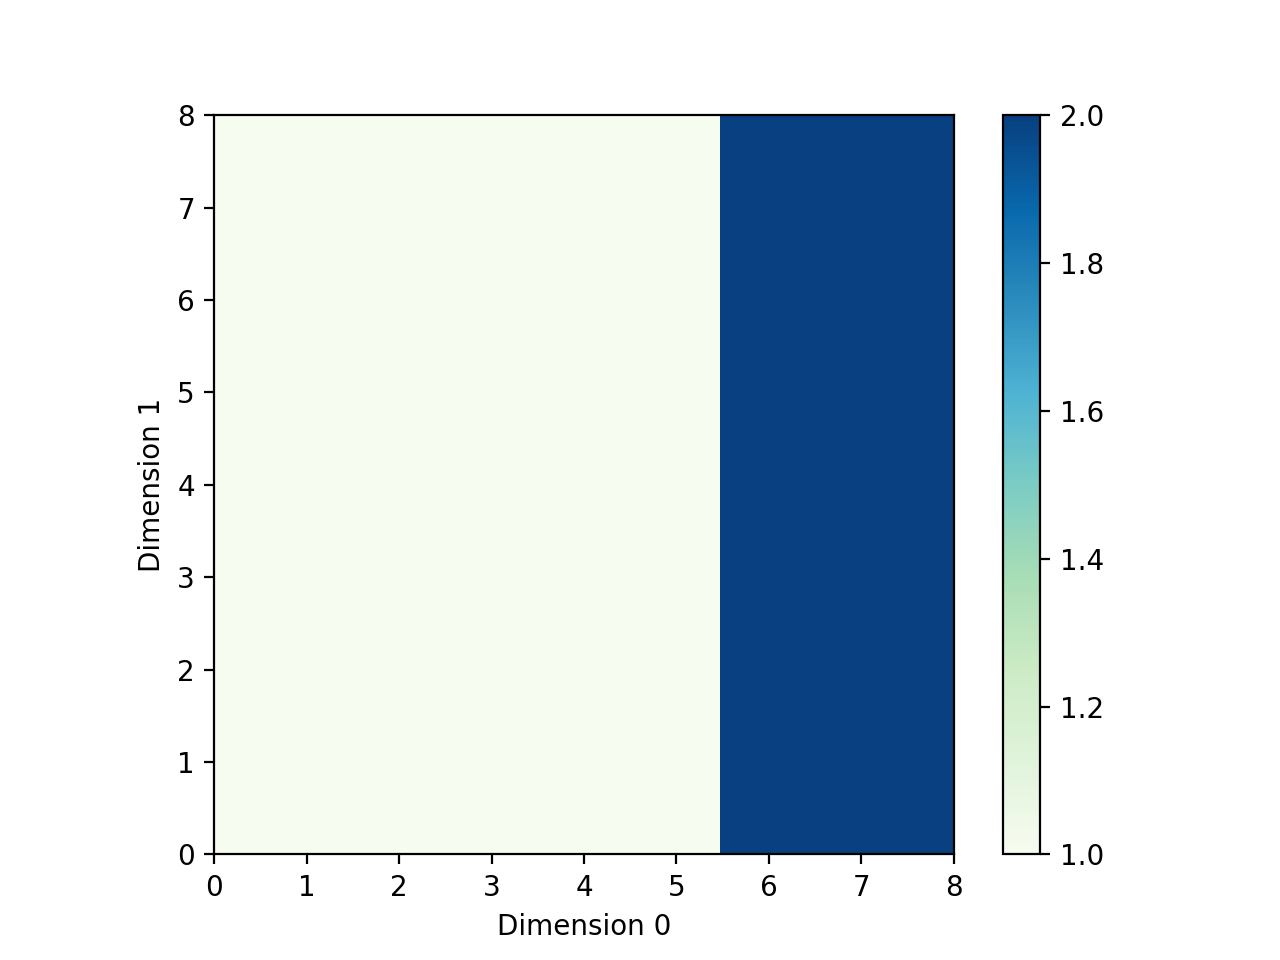
\includegraphics[width=0.6\textwidth] {Tree}}
\subfigure[Adaboost]{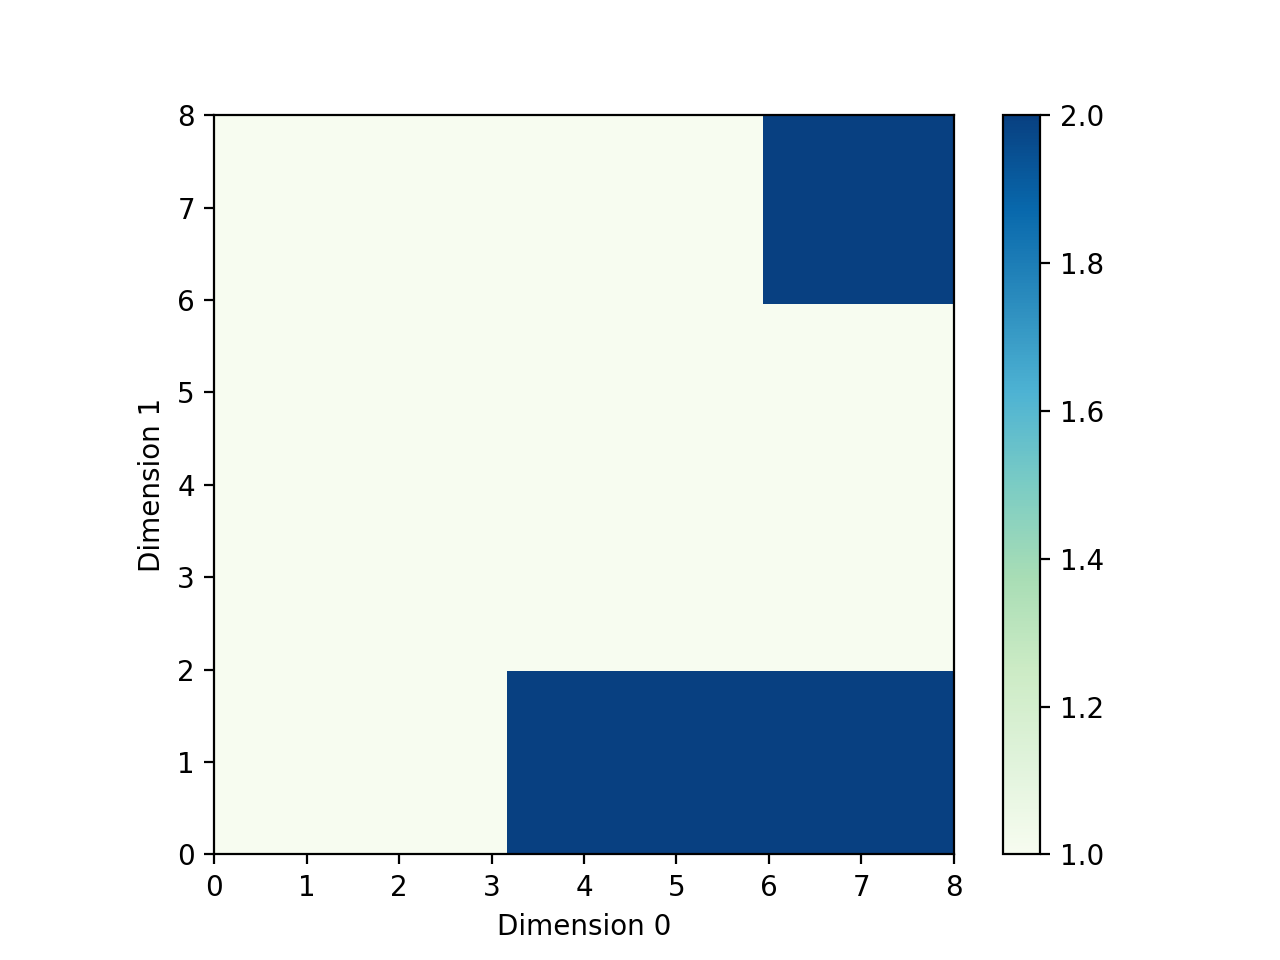
\includegraphics[width=0.6\textwidth] {Ada}}
\caption{弱識別器と強識別器の識別領域} 
\end{figure}


\end{document}